%%%%%%%%%%%%%%%%%%%%%%%%%%%%%%%%%%%%%%%%%%%%%%%%%%%%%%%%%%%%%%%%%%%%%%

%%% Preamble
\documentclass[	DIV=calc,%
							paper=letter,%
							fontsize=12pt%,%
							%twocolumn
                            ]{scrartcl}	 					% KOMA-article class

\usepackage{lipsum}													% Package to create dummy text

\usepackage[english]{babel}	
\selectlanguage{english}
% English language/hyphenation
\usepackage[protrusion=true,expansion=true]{microtype}				% Better typography
\usepackage{amsmath,amsfonts,amsthm,mathabx}					% Math packages
\usepackage[pdftex]{graphicx}									% Enable pdflatex
\usepackage[svgnames]{xcolor}									% Enabling colors by their 'svgnames'
\usepackage[hang, small,labelfont=bf,up,textfont=it,up]{caption}	% Custom captions under/above floats
\usepackage{epstopdf}												% Converts .eps to .pdf
\usepackage{subfig}													% Subfigures
\usepackage{booktabs}												% Nicer tables
\usepackage{fix-cm}													% Custom fontsizes
\usepackage{cite}
\usepackage{capt-of}
\usepackage[pdftex=false,colorlinks=true,plainpages=true,citecolor=black,linkcolor=black]{hyperref}


%%% Custom sectioning (sectsty package)
\usepackage{sectsty}													% Custom sectioning (see below)
\allsectionsfont{%															% Change font of al section commands
	\usefont{OT1}{phv}{b}{n}%										% bch-b-n: CharterBT-Bold font
	}

\sectionfont{%																% Change font of \section command
	\usefont{OT1}{phv}{b}{n}%										% bch-b-n: CharterBT-Bold font
	}



%%% Headers and footers
\usepackage{fancyhdr}												% Needed to define custom headers/footers
	\pagestyle{fancy}														% Enabling the custom headers/footers
\usepackage{lastpage}	

% Header (empty)
\lhead{}
\chead{}
\rhead{}
% Footer (you may change this to your own needs)
\lfoot{\footnotesize \texttt{Intelligent Wallet} }
\cfoot{}
\rfoot{\footnotesize Page \thepage\ of \pageref{LastPage}}	% "Page 1 of 2"
\renewcommand{\headrulewidth}{0.0pt}
\renewcommand{\footrulewidth}{0.4pt}
\addto\captionsenglish{\renewcommand{\figurename}{Figure}}
\addto\captionsenglish{\renewcommand{\tablename}{Table}}
\addto\captionsenglish{\renewcommand{\refname}{References}} 


%%% Creating an initial of the very first character of the content
\usepackage{lettrine}
\newcommand{\initial}[1]{%
     \lettrine[lines=3,lhang=0.3,nindent=0em]{
     				\color{DarkGoldenrod}
     				{\textsf{#1}}}{}}



%%% Title, author and date metadata
\usepackage{titling}															% For custom titles

\newcommand{\HorRule}{\color{DarkGoldenrod}%			% Creating a horizontal rule
									  	\rule{\linewidth}{1pt}%
										}

\pretitle{\vspace{-30pt} \begin{flushleft} \HorRule 
				\fontsize{35}{35} \usefont{OT1}{phv}{b}{n} \color{DarkRed} \selectfont 
				}
\title{Intelligent Wallet}					% Title of your article goes here
\posttitle{\par\end{flushleft}\vskip 0.5em}

\preauthor{\begin{flushleft}
					\large \lineskip 0.5em \usefont{OT1}{phv}{b}{sl} \color{DarkRed}}
\author{}											% Author name goes here
\postauthor{\footnotesize \usefont{OT1}{phv}{m}{sl} \color{Black} 
											% Institution of author
					\par\end{flushleft}\HorRule}

\date{}																				% No date

\providecommand{\keywords}[1]
{
  \small	
  \textbf{\textit{Keywords---}} #1
}

%%% Begin document
\begin{document}
\maketitle


\newpage
\begin{abstract}
	
{A chatbot is a technology capable of simulating a human being conversation through a conversational interface. By the use of Artificial Intelligence (AI) and Machine Learning (ML) techniques, it automates the responses to a user through the exchange of messages in what the user perceives as natural language and executes tasks that are designed to transform the experience of the users.

Among diverse types of activities, users might be able to make a reservation   at a restaurant, slide through the product carousels and make a purchase; be notified about canceling a flight to change the ticket at that precise moment and even trace the luggage; it also might be possible to learn how to trade and manage cryptocurrencies through chatbots.

In this paper a design for a cryptocurrency chatbot based on emotions is provided. It answers to queries related to trading and use the human interaction to recognize emotions and predict purchasing intents.}

\end{abstract}

\keywords{chatbot, Artificial Intelligence, Machine Learning, Natural Language Processing, cryptocurrency, emotions}

\newpage
\tableofcontents
\newpage
\listoffigures
\newpage

\thispagestyle{fancy} 			% Enabling the custom headers/footers for the first page 
% The first character should be within \initial{}

\section{\label{sec:level1}Introduction}

Chatbots are the result of an evolution of more than 30 years. The first conversational bot was Eliza, invented in the 1960s by the German Joseph Wiezenbaum in the laboratory of Artificial Intelligence from the Massachusetts Institute of Technology (MIT), in U.S. In the 1990s, companies implemented telephone IVRs, systems of interactive voice response. Today, users demand 24/7 attention, immediate, digestible and useful. For the companies this requirement has become an opportunity to improve their customer services models and experience strategies. 


Chatbots are positioned as main players of innovation. Using chatbots has become an option that more and more companies are using to provide an additional service to their customers. In the past few months, a hype about this topic has been developed and according to Credence Research, chatbots are going to be a key piece of automation for 2019 and Gartner estimates that more than 85\% of the service centers client, will be operated by bots in 2020.
\section{\label{sec:level1}Creating User’s Engagement}

Chatbots work most likely humans handle technical support. The chatbot is the medium responding when a customer starts a conversation looking for support. For example, if a trader requests the price of Litecoin, using the information available, the chatbot would immediately respond in the same way as a human would: “George, you recently asked me about Litecoin. Would you like to trade Litecoin, Bitcoin, Ether and 100+ more cryptocurrencies on our new multi-asset trading platform? Click here to find out more”.


A Chatbot can create engagement between business and customers without human interaction. This engagement can be created through small talks: it could be started by sending alerts, for example: “Notify me when a Bitcoin is less than \$7000”; if this event occurs, the chatbot notifies the user adding a call to action “Would you like to trade the Bitcoin now?”. It could broadcast general messages to a wider audience to crate engagement: “Federal Reserve Governor speaks at 3:15pm EST, don’t forget to top up your account!”
 
Chatbots could also be connected to a trading platform where the chatbot analyze the trader’s exposure to the market and warn of potential threats, for example, “The U.S. Nonfarm Payrolls are out today at 13:30 GMT, which may cause significant volatility. Would you like to manage your positions now?”
 
With the past of the time the chatbot can become smarter by learning from the user’s deposit history, open positions and margin requirements so it can make calls-to-action more targeted: \textit{“Your equity is \$1040.34. Should EUR/USD drop more than 100 pips, your position “\#123 Buy 1 lot EUR/USD @ 1.12345” will be liquidated. Would you like to top up your account to avoid this? The suggested amount is \$450”}.

\section{\label{sec:level1}Trade and Transactions via Chat}

Currently the push notifications are the way to do outbound marketing.
Brands can schedule promotions and launch them without customization as long day Users are full of notifications out of context.


The chatbots respond to the micromomentos of the people and their level of understanding allows you to make predictions of purchase. For example, if a person bought tickets to watch his favorite team's football game, the chatbot can notify you about the following entries and propose the best seats, suggest that you purchase the special edition cap or you may notice how to get to the stadium, mention nearby parking lots and can even buy food and beverages with a special promotion before reaching the event.


All without having to leave your messaging platform. It will not be necessary that he resorts to the app to buy his tickets or to the web site to consult the prices of souvenirs, or open the browser to trace your route.

\section{\label{sec:level1}Functionality}

Intelligent Wallet ™ works so that the client specifies one or multiple “Intents” that correspond to a single action or a question the user wants to do. A show.coins intent could, for example, display the best coin to trade during the day for the user. Examples, like “What’s the bullish?” or “Give me the bullish.” The platform can then use these examples with machine learning to match users queries to the correct intent.

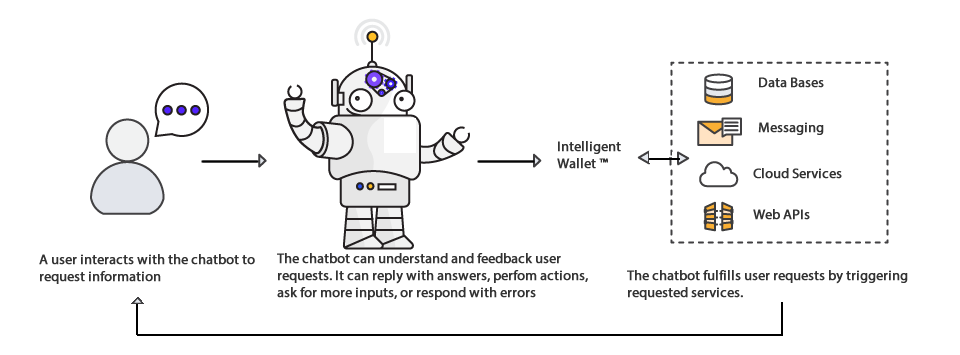
\includegraphics[scale=0.40]{img/Chatbot.png}\vspace*{1cm}

Instead of browsing a website, you will have a conversation with the bot, mirroring the type of experience you would get when you go into the complete platform.

\section{\label{sec:level1}Crypto Currency Services}
Through the platform two main services can be provided\: Investment Advice and Information Management. The first one has to do with the delivery of recommendations or personalized advices to our users, which suggest the investment decision making about the cryptocurrency. The second one provides Market Information and Individual Account balances.


In order to provide the Investment Advice service Intelligent Wallet ™ requires you to fill some questionnaires  which lead us to determine your experience with finance, cryptocurrencies,situation and financial capabilities , the investment objective with the finality of give you suitable advices according to your investment needs.

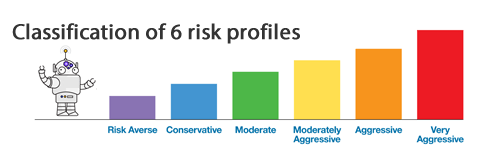
\includegraphics[scale=0.65]{img/risks.png}\vspace*{1.5cm}

\section{\label{sec:level1}Conclusion}
Sophisticated chatbots break new ground in conversion and activation of prospects into sales. Being a diligent conversational partner, this AI remembers the history of the dialog and is continuously self-learning. Thus, a chatbot can connect with a user on a more intimate level, it has the ability to get under a traders’ skin by adding value that improves their day-to-day lives. However, only a chatbot with a well-designed architecture and advanced functionality can enrich a company’s communications. \cite{Barbara_CL2018}

Chatbots still remain an underrated channel these days among brokerages, it is an appropriate time to explore whether your business may need one.

\newpage
\bibliography{References}
\bibliographystyle{IEEEtran}
\end{document}